% Human-Centered Data Collection for Machine Learning: Lessons from Survey Research
% AAPOR Conference Short Course, May 12, 2025, Los Angeles
% Stephanie Eckman & Frauke Kreuter

\documentclass[aspectratio=169,11pt]{beamer}
\usetheme{metropolis}

% ── Packages ──────────────────────────────────────────────────
\usepackage{booktabs}
\usepackage{graphicx}
\usepackage{tikz}
\usetikzlibrary{arrows.meta, positioning, shapes.geometric, calc}
\usepackage{natbib}
\usepackage{hyperref}
\usepackage{appendixnumberbeamer}
\usepackage{xcolor}
\usepackage{amsmath}
\usepackage{tabularx}
\usepackage{multirow}

% ── Color definitions ─────────────────────────────────────────
\definecolor{mLightBrown}{HTML}{EB811B}  % Metropolis accent
\definecolor{mDarkTeal}{HTML}{23373B}    % Metropolis dark
\definecolor{alertcol}{HTML}{BF616A}     % For warnings/emphasis
\definecolor{successcol}{HTML}{A3BE8C}   % For positive points
\definecolor{neutralcol}{HTML}{5E81AC}   % For neutral highlights
\definecolor{lightbg}{HTML}{ECEFF4}      % Light background for boxes

% ── Metropolis customization ──────────────────────────────────
\setbeamercolor{frametitle}{bg=mDarkTeal}
\setbeamerfont{frametitle}{size=\large}
\setbeamertemplate{frame numbering}[fraction]

% ── Citation style ────────────────────────────────────────────
\bibliographystyle{plainnat}
\setcitestyle{authoryear,round}

% ── Metadata ──────────────────────────────────────────────────
\title{Human-Centered Data Collection\\for Machine Learning}
\subtitle{Lessons from Survey Research}
\author{Stephanie Eckman \and Frauke Kreuter}
\institute{AAPOR Conference Short Course}
\date{May 12, 2025}

\begin{document}

% ══════════════════════════════════════════════════════════════
% SECTION 1: Introduction
% ══════════════════════════════════════════════════════════════

\maketitle

% ── Roadmap ───────────────────────────────────────────────────
\begin{frame}{Four hours, one argument}
\begin{enumerate}
  \item Introduction: Why data quality matters
  \item Survey data collection basics
  \item Training data collection
  \item \textbf{Measurement:} Are the labels correct?
  \item \textbf{Representation:} Who labels?
  \item \textbf{Sampling:} Which instances to label?
  \item Ethics of data work
  \item Practical advice
  \item Discussion
\end{enumerate}

\vspace{1em}
\small We will take breaks. Ask questions anytime.
\end{frame}

% ── Who we are ────────────────────────────────────────────────
\begin{frame}{Who we are}
\textbf{Stephanie Eckman} -- University of Maryland\\[0.5em]
Survey methodologist studying how data collection design\\
affects data quality -- now applied to ML training data.

\vspace{1.5em}

\textbf{Frauke Kreuter} -- LMU Munich / University of Maryland\\[0.5em]
Survey methodology, data science, and the intersection\\
of social science methods with machine learning.
\end{frame}

% ── Why this course ───────────────────────────────────────────
\begin{frame}{ML models are only as good as their training data}

\begin{quote}
``Everyone wants to do the model work, not the data work.''
\end{quote}

\vspace{0.5em}
\hfill --- \citet{sambasivan2021everyone}

\vspace{1.5em}

Data quality problems are the most common cause of\\
ML system failures in production.

\vspace{0.5em}
\hfill \citep{sculley2015hidden}
\end{frame}

% ── Data-centric AI ──────────────────────────────────────────
\begin{frame}{The shift to data-centric AI}

Traditional ML: fix the data, iterate on the \textbf{model}.

\vspace{1em}

Data-centric AI: fix the model, iterate on the \textbf{data}.

\vspace{1.5em}

Survey researchers have been iterating on data quality\\
for \textbf{decades}. We have tools for this.

\vspace{1em}
\hfill \citep{ng2021data}
\end{frame}

% ── What survey research brings ──────────────────────────────
\begin{frame}{Survey researchers bring a unique perspective}
\begin{itemize}
  \item Frameworks for thinking about data quality (Total Survey Error)
  \item Experience designing instruments that minimize bias
  \item Understanding of how question design affects responses
  \item Methods for assessing and reducing measurement error
  \item Decades of research on who responds and why it matters
\end{itemize}
\end{frame}

% ══════════════════════════════════════════════════════════════
% SECTION 2: Survey Data Collection Basics
% ══════════════════════════════════════════════════════════════

\section{Survey Data Collection Basics}

\begin{frame}{The Total Survey Error framework}

Two families of error:

\vspace{1em}

\begin{columns}[T]
\begin{column}{0.45\textwidth}
\textbf{Measurement}\\[0.5em]
Is the answer correct?\\[0.3em]
\small Validity, measurement error,\\
processing error
\end{column}

\begin{column}{0.45\textwidth}
\textbf{Representation}\\[0.5em]
Who answered?\\[0.3em]
\small Coverage, sampling,\\
nonresponse, adjustment
\end{column}
\end{columns}

\vspace{1.5em}

This framework organizes our entire course.
\end{frame}

% ── TSE diagram ──────────────────────────────────────────────
\begin{frame}{Total Survey Error: the full picture}
\begin{center}
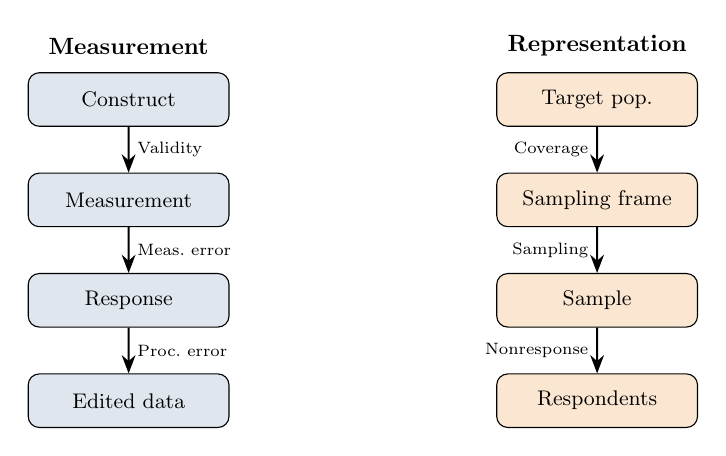
\begin{tikzpicture}[
  box/.style={draw, rounded corners, minimum width=3cm, minimum height=0.8cm, align=center, font=\small},
  arrow/.style={-Stealth, thick},
  scale=0.85, transform shape
]
% Measurement side
\node[box, fill=neutralcol!20] (construct) at (-3.5, 3) {Construct};
\node[box, fill=neutralcol!20] (measure) at (-3.5, 1.5) {Measurement};
\node[box, fill=neutralcol!20] (response) at (-3.5, 0) {Response};
\node[box, fill=neutralcol!20] (edited) at (-3.5, -1.5) {Edited data};

\draw[arrow] (construct) -- node[right, font=\scriptsize] {Validity} (measure);
\draw[arrow] (measure) -- node[right, font=\scriptsize] {Meas.\ error} (response);
\draw[arrow] (response) -- node[right, font=\scriptsize] {Proc.\ error} (edited);

% Representation side
\node[box, fill=mLightBrown!20] (target) at (3.5, 3) {Target pop.};
\node[box, fill=mLightBrown!20] (frame) at (3.5, 1.5) {Sampling frame};
\node[box, fill=mLightBrown!20] (sample) at (3.5, 0) {Sample};
\node[box, fill=mLightBrown!20] (respondents) at (3.5, -1.5) {Respondents};

\draw[arrow] (target) -- node[left, font=\scriptsize] {Coverage} (frame);
\draw[arrow] (frame) -- node[left, font=\scriptsize] {Sampling} (sample);
\draw[arrow] (sample) -- node[left, font=\scriptsize] {Nonresponse} (respondents);

% Labels
\node[font=\bfseries] at (-3.5, 3.8) {Measurement};
\node[font=\bfseries] at (3.5, 3.8) {Representation};
\end{tikzpicture}
\end{center}
\end{frame}

% ── Measurement side ─────────────────────────────────────────
\begin{frame}{Measurement: three sources of error}
\begin{description}
  \item[Validity] Does the question measure what we intend?
  \item[Measurement error] Systematic or random deviations from the true value
  \item[Processing error] Errors introduced during coding, editing, or data entry
\end{description}

\vspace{1em}

Each of these has a direct analogue in training data collection.
\end{frame}

% ── Representation side ──────────────────────────────────────
\begin{frame}{Representation: three sources of error}
\begin{description}
  \item[Coverage] Who is missing from the frame?
  \item[Sampling] Which units are selected?
  \item[Nonresponse] Who refuses or is unreachable?
\end{description}

\vspace{1em}

Each of these has a direct analogue in training data collection.
\end{frame}

% ── Cognitive model ──────────────────────────────────────────
\begin{frame}{How survey respondents answer questions}

\textbf{The cognitive model of survey response:}

\vspace{1em}

\begin{center}
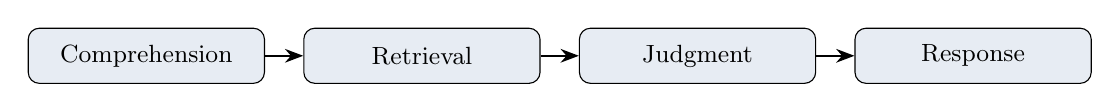
\begin{tikzpicture}[
  stagenode/.style={draw, rounded corners, fill=neutralcol!15, minimum width=3cm, minimum height=0.7cm, align=center, font=\small},
  arrow/.style={-Stealth, thick}
]
\node[stagenode] (comp) at (0,0) {Comprehension};
\node[stagenode] (recall) at (3.5,0) {Retrieval};
\node[stagenode] (judge) at (7,0) {Judgment};
\node[stagenode] (resp) at (10.5,0) {Response};

\draw[arrow] (comp) -- (recall);
\draw[arrow] (recall) -- (judge);
\draw[arrow] (judge) -- (resp);
\end{tikzpicture}
\end{center}

\vspace{1em}

Errors can enter at \textbf{every stage}.\\
The same model applies to annotators labeling data.
\end{frame}

% ══════════════════════════════════════════════════════════════
% SECTION 3: Training Data Collection
% ══════════════════════════════════════════════════════════════

\section{Training Data Collection}

\begin{frame}{Where does training data come from?}
\begin{enumerate}
  \item \textbf{Found data} -- web scraping, social media, government records
  \item \textbf{Elicited data} -- surveys, experiments
  \item \textbf{Human-labeled data} -- human annotators assign labels to items
\end{enumerate}

\vspace{1em}

This course focuses on \textbf{human-labeled data}:\\
the labels that teach ML models what is ``correct.''
\end{frame}

% ── What labeling looks like ─────────────────────────────────
\begin{frame}{What does labeling look like in practice?}
Examples of labeling tasks:
\begin{itemize}
  \item \textbf{Text classification:} Is this tweet hate speech? Offensive? Neither?
  \item \textbf{Image classification:} Does this image contain a pedestrian?
  \item \textbf{Named entity recognition:} Mark all person names in this text
  \item \textbf{RLHF:} Which of two model responses is better?
  \item \textbf{Relevance:} Is this search result relevant to the query?
\end{itemize}

\vspace{1em}

Each task has \textbf{design choices} that affect label quality.
\end{frame}

% ── The human side ───────────────────────────────────────────
\begin{frame}{Labelers are people, not machines}

Behind every training dataset are \textbf{human decisions}.

\vspace{1em}

\begin{itemize}
  \item Annotators interpret guidelines
  \item They bring their own backgrounds and biases
  \item They experience fatigue, boredom, and confusion
  \item They are affected by task design, pay, and working conditions
\end{itemize}

\vspace{1em}

Sound familiar? These are the same issues survey\\
researchers study in \textbf{interviewers} and \textbf{respondents}.
\end{frame}

% ── TSE applied to training data ─────────────────────────────
\begin{frame}{Total Survey Error maps onto training data}
\begin{center}
\small
\begin{tabular}{lll}
\toprule
\textbf{TSE Concept} & \textbf{Survey} & \textbf{Training Data} \\
\midrule
Measurement & Question $\to$ answer & Task $\to$ label \\
Validity & Q.\ measures construct? & Label reflects concept? \\
Meas.\ error & Interviewer effects & Annotator effects \\
Representation & Who responds? & Who labels? \\
Coverage & Frame misses units & Pool misses instances \\
Sampling & Which units selected? & Which instances labeled? \\
Nonresponse & Who refuses? & Who drops out/skips? \\
\bottomrule
\end{tabular}
\end{center}
\end{frame}

% ══════════════════════════════════════════════════════════════
% SECTION 4: Measurement -- Are the Labels Correct?
% ══════════════════════════════════════════════════════════════

\section{Measurement: Are the Labels Correct?}

\begin{frame}{The construct-to-label path is long}

\begin{center}
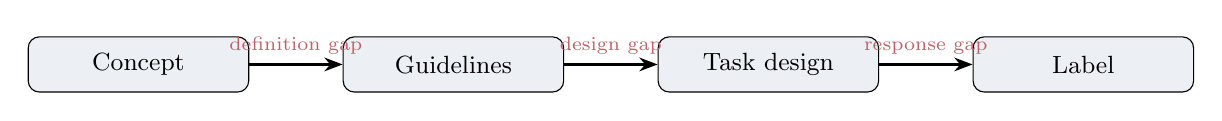
\begin{tikzpicture}[
  box/.style={draw, rounded corners, fill=lightbg, minimum width=2.8cm, minimum height=0.7cm, align=center, font=\small},
  arrow/.style={-Stealth, thick},
  gap/.style={font=\scriptsize, text=alertcol}
]
\node[box] (concept) at (0,0) {Concept};
\node[box] (guidelines) at (4,0) {Guidelines};
\node[box] (task) at (8,0) {Task design};
\node[box] (label) at (12,0) {Label};

\draw[arrow] (concept) -- node[above, gap] {definition gap} (guidelines);
\draw[arrow] (guidelines) -- node[above, gap] {design gap} (task);
\draw[arrow] (task) -- node[above, gap] {response gap} (label);
\end{tikzpicture}
\end{center}

\vspace{1em}

At each step, error can enter.\\
Survey researchers know this path well.
\end{frame}

% ── Annotation design affects labels ─────────────────────────
\begin{frame}{Annotation design affects the labels you get}

\citet{kern2023annotation} ran an experiment:\\[0.5em]

\textbf{Same tweets}, different annotation designs $\to$ \textbf{different labels}.

\vspace{1em}

Design choices that mattered:
\begin{itemize}
  \item Number of response categories
  \item Whether ``offensive'' was a separate category
  \item Task framing and instructions
\end{itemize}

\vspace{1em}

The label is not a property of the text.\\
It is a product of the \textbf{measurement instrument}.

\vspace{0.5em}
\hfill \small \textit{Hate speech / offensive language classification}
\end{frame}

% ── Details of Kern et al ────────────────────────────────────
\begin{frame}{Different instruments, different ``ground truth''}

% TODO: Include figure from Kern et al 2023 showing experimental conditions
% \includegraphics[width=\textwidth]{figures/kern-et-al-conditions.pdf}

\citet{kern2023annotation} tested multiple annotation designs\\
for the \textbf{same} hate speech classification task.

\vspace{1em}

Key finding: Models trained on labels from different designs\\
had \textbf{different accuracy levels} and \textbf{different error patterns}.

\vspace{1em}

\textbf{Implication:} The ``ground truth'' depends on how you ask.
\end{frame}

% ── Pre-labeling / automation bias ───────────────────────────
\begin{frame}{Pre-labeling can introduce automation bias}

\citet{beck2025pre} studied what happens when annotators\\
see \textbf{model-suggested labels} before making their own judgment.

\vspace{1em}

\begin{itemize}
  \item Annotators anchor on the pre-label
  \item They are less likely to disagree with the suggestion
  \item This is \textbf{automation bias} -- the same phenomenon\\
        documented in aviation, medicine, and survey editing
\end{itemize}

\vspace{1em}

Pre-labeling saves time but may \textbf{reduce label independence}.
\end{frame}

% ── Order effects ────────────────────────────────────────────
\begin{frame}{The order of items affects labels}

\citet{beck2024order} found that the \textbf{sequence} in which\\
annotators see items affects their labeling decisions.

\vspace{1em}

Survey researchers call these \textbf{context effects}:
\begin{itemize}
  \item Assimilation: current judgment pulled toward previous item
  \item Contrast: current judgment pushed away from previous item
  \item Fatigue: quality degrades over the session
\end{itemize}

\vspace{1em}

\textbf{Implication:} Randomize item order across annotators.
\end{frame}

% ── Question design lessons ──────────────────────────────────
\begin{frame}{Lessons from 80 years of question design research}

Survey research offers tested principles:

\vspace{1em}

\begin{itemize}
  \item Avoid ambiguous terms (define ``hate speech'')
  \item Provide balanced response options
  \item Use consistent scales across items
  \item Avoid double-barreled questions
  \item Pretest the instrument before full deployment
\end{itemize}

\vspace{1em}

\hfill \citep{krosnick2010question, sudman1982asking}
\end{frame}

% ── Discussion break ─────────────────────────────────────────
\begin{frame}[standout]
Discussion
\end{frame}

\begin{frame}{Discussion: Measurement}

\begin{enumerate}
  \item Think of a labeling task in your work.\\
        What design choices could affect the labels?

  \vspace{1em}

  \item Have you encountered situations where the ``ground truth''\\
        depended on how the question was asked?
\end{enumerate}
\end{frame}

% ══════════════════════════════════════════════════════════════
% SECTION 5: Representation -- Who Labels?
% ══════════════════════════════════════════════════════════════

\section{Representation: Who Labels?}

\begin{frame}{Who provides the labels?}
\begin{description}
  \item[Domain experts] Doctors, lawyers, linguists -- high quality, expensive, scarce
  \item[Trained annotators] Hired and trained for the task -- moderate cost
  \item[Crowdworkers] MTurk, Prolific, Scale AI -- cheap, fast, variable quality
  \item[The researchers themselves] Small scale, potential bias
  \item[LLMs] Increasingly used, but with systematic biases
\end{description}

\vspace{1em}

Each choice shapes the labels -- and the resulting model.
\end{frame}

% ── Nonresponse framework ────────────────────────────────────
\begin{frame}{Nonresponse bias applies to labeling too}

In surveys, nonresponse bias arises when:\\
people who respond differ from people who don't.

\vspace{1em}

In labeling:
\begin{itemize}
  \item Which annotators accept the task? (self-selection)
  \item Which annotators complete it? (attrition)
  \item Which annotators pass quality checks? (filtering)
\end{itemize}

\vspace{1em}

At each stage, the remaining annotators\\
may \textbf{differ systematically} from those who left.
\end{frame}

% ── Annotator demographics affect labels ─────────────────────
\begin{frame}{Labeler characteristics affect the labels}

\textbf{Annotator demographics predict label distributions.}

\vspace{1em}

\citet{otterbacher2018investigating}: Annotator gender and age\\
affected how they labeled stereotype content in image search.

\vspace{1em}

\citet{alkuwatly2020identifying}: Annotator demographics\\
predicted systematic differences in toxicity labels.

\vspace{1em}

This is not noise -- it is \textbf{systematic measurement error}\\
correlated with annotator characteristics.
\end{frame}

% ── Labeler diversity ────────────────────────────────────────
\begin{frame}{Labeler diversity affects model behavior}

If your annotators are \textbf{demographically homogeneous}:
\begin{itemize}
  \item Labels reflect one group's perspective
  \item Models learn that perspective as ``ground truth''
  \item Performance degrades for underrepresented groups
\end{itemize}

\vspace{1em}

Survey researchers understand this:\\
a sample must \textbf{represent} the target population.

\vspace{1em}

But who is the ``target population'' for annotators?
\end{frame}

% ── Can LLMs replace human labelers? ─────────────────────────
\begin{frame}{Can LLMs replace human labelers?}

Increasingly, teams use GPT-4 or similar models to generate labels.

\vspace{1em}

Risks:
\begin{itemize}
  \item LLMs reproduce biases in their training data
  \item \textbf{Model collapse:} models trained on model-generated data\\
        lose diversity over generations \citep{shumailov2023curse}
  \item LLM labels are not independent of each other
  \item We lose the \textbf{signal in human disagreement}
\end{itemize}

\vspace{1em}

LLM labels may be useful, but they are not a free replacement\\
for thoughtful human annotation.
\end{frame}

% ── Discussion break ─────────────────────────────────────────
\begin{frame}[standout]
Discussion
\end{frame}

\begin{frame}{Discussion: Representation}

\begin{enumerate}
  \item Who labels in your organization?\\
        How were they recruited and selected?

  \vspace{1em}

  \item If labeler characteristics affect labels,\\
        what does ``representative'' mean for an annotator pool?
\end{enumerate}
\end{frame}

% ══════════════════════════════════════════════════════════════
% SECTION 6: Sampling -- Which Instances to Label?
% ══════════════════════════════════════════════════════════════

\section{Sampling: Which Instances to Label?}

\begin{frame}{You can't label everything}

Labeling is expensive. You must choose which instances to label.

\vspace{1em}

\textbf{Options:}
\begin{itemize}
  \item Simple random sampling from the pool
  \item Uncertainty sampling (where the model is confused)
  \item Diversity sampling (cover the feature space)
  \item Active learning (iterative, model-guided selection)
\end{itemize}

\vspace{1em}

\hfill \citep{monarch2021human}
\end{frame}

% ── How many labels ──────────────────────────────────────────
\begin{frame}{How many labels do you need?}

In surveys: sample size is determined \textbf{before} data collection\\
(power analysis, margin of error, design effect).

\vspace{1em}

In active learning: sample size is determined \textbf{during} collection\\
(stop when accuracy plateaus or budget runs out).

\vspace{1em}

There is no universal formula.\\
It depends on task complexity, class balance, and model architecture.
\end{frame}

% ── Section divider: sampling comparison ─────────────────────
\begin{frame}[standout]
Sampling for Labels\\vs.\ Sampling for Surveys
\end{frame}

% ── You know sampling ────────────────────────────────────────
\begin{frame}{You know sampling -- but ML uses these words differently}

You have spent careers thinking about:\\
probability sampling, stratification, clustering, sample size.

\vspace{1em}

The active learning literature uses \textbf{the same vocabulary}\\
but \textbf{shifts the meanings}.

\vspace{1em}

The next several slides map the terminology precisely.\\
The collisions are not minor -- they are fundamental.
\end{frame}

% ── Monarch's taxonomy ───────────────────────────────────────
\begin{frame}{Monarch's four types of ``diversity sampling''}

\citet{monarch2021human} uses \textbf{diversity sampling} as an umbrella\\
for all non-uncertainty-based sampling:

\vspace{1em}

\begin{enumerate}
  \item \textbf{Model-based outliers} -- items far from training data in feature space
  \item \textbf{Cluster-based sampling} -- k-means on features, sample from each cluster
  \item \textbf{Representative sampling} -- sample items that look like the unlabeled pool
  \item \textbf{Real-world diversity} -- ensure demographic groups are covered
\end{enumerate}

\vspace{1em}

He notes: ``diversity sampling goes by different names in different\\
fields, such as representative sampling, stratified sampling.''
\end{frame}

% ── Terminology collision table ──────────────────────────────
\begin{frame}{The same words mean different things}
\begin{center}
\footnotesize
\begin{tabularx}{\textwidth}{lXX}
\toprule
\textbf{Term} & \textbf{Survey Sampling} & \textbf{Active Learning} \\
\midrule
Stratification & Non-overlapping subgroups of the \textit{population}; sample from each stratum &
  Bin items by \textit{model confidence} or \textit{predicted label}; sample from each bin \\[0.8em]
Clustering & Select \textit{groups of units} (schools, blocks) as PSUs for cost efficiency &
  Group \textit{data points} by similarity in feature space; sample near centroids \\[0.8em]
Representative & Sample mirrors the \textit{population} via probability sampling + weighting &
  Sample mirrors the \textit{unlabeled pool} in feature space \\[0.8em]
Diversity & Via stratification; ensure population subgroups represented &
  Umbrella term for all non-uncertainty sampling \\
\bottomrule
\end{tabularx}
\end{center}
\end{frame}

% ── Stratification ───────────────────────────────────────────
\begin{frame}{``Stratified sampling'' means something different in ML}

\textbf{In surveys:}\\
Define non-overlapping subgroups of a \textit{population} \textbf{before}\\
data collection. Sample from each stratum with known\\
inclusion probabilities.

\vspace{1em}

\textbf{In active learning:}\\
Bin unlabeled items by \textit{model confidence} or \textit{predicted label}.\\
Sample equal amounts from each bin to avoid oversampling\\
easy, high-confidence cases.

\vspace{1em}

Strata in AL are defined by \textbf{model output}, not population\\
characteristics. They have no inclusion probabilities.\\
And they \textbf{change} every time the model retrains.
\end{frame}

% ── Stratification example ───────────────────────────────────
\begin{frame}{Example: Monarch's ``stratify by confidence''}

\begin{center}
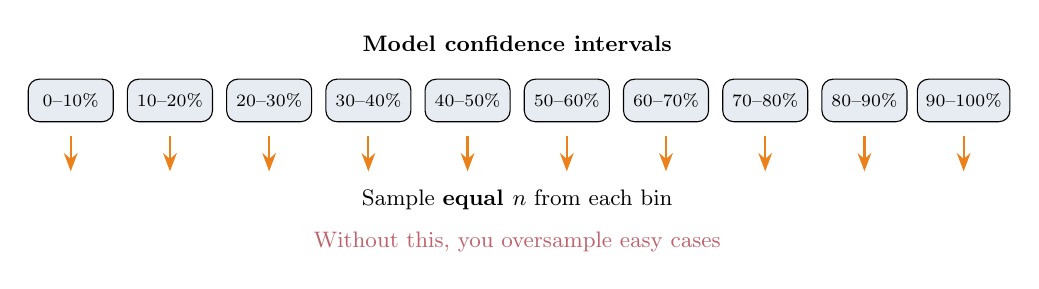
\begin{tikzpicture}[
  bin/.style={draw, rounded corners, fill=neutralcol!15, minimum width=1.2cm, minimum height=0.6cm, align=center, font=\scriptsize},
  scale=0.9, transform shape
]
% Confidence bins
\foreach \i/\label in {0/0--10\%, 1/10--20\%, 2/20--30\%, 3/30--40\%, 4/40--50\%, 5/50--60\%, 6/60--70\%, 7/70--80\%, 8/80--90\%, 9/90--100\%} {
  \node[bin] at (\i*1.4, 0) {\label};
}

% Equal sampling arrows
\foreach \i in {0,...,9} {
  \draw[-Stealth, thick, mLightBrown] (\i*1.4, -0.5) -- (\i*1.4, -1.0);
}

\node[font=\small] at (6.3, -1.4) {Sample \textbf{equal $n$} from each bin};
\node[font=\small, text=alertcol] at (6.3, -2.0) {Without this, you oversample easy cases};

% Label
\node[font=\small\bfseries] at (6.3, 0.8) {Model confidence intervals};
\end{tikzpicture}
\end{center}

\vspace{0.5em}

A survey statistician would call this \textbf{post-stratification}\\
on a model-generated variable -- not stratified sampling.

\hfill \citep{monarch2021human}
\end{frame}

% ── Clustering ───────────────────────────────────────────────
\begin{frame}{``Clustering'' means something different in ML}

\textbf{In surveys:}\\
Select \textit{groups of operational units} (schools, blocks,\\
households) as primary sampling units for \textbf{cost efficiency}.\\
Then survey units within selected clusters.

\vspace{1em}

\textbf{In active learning:}\\
Run k-means or similar on \textit{feature-space embeddings}.\\
Sample items nearest each centroid to maximize\\
\textbf{coverage of the feature space}.

\vspace{1em}

Survey clusters are defined by \textbf{geography and logistics}.\\
AL clusters are defined by \textbf{similarity in a learned representation}.\\
Same word, completely different unit of analysis and purpose.
\end{frame}

% ── Representative ───────────────────────────────────────────
\begin{frame}{``Representative'' means something different in ML}

\textbf{In surveys:}\\
A sample is representative when it mirrors the \textit{population}\\
via probability sampling and appropriate weighting.

\vspace{1em}

\textbf{In active learning:}\\
A sample is ``representative'' when it mirrors the\\
\textit{unlabeled data pool} in feature space.

\vspace{1em}

\textbf{Key difference:}\\
AL has no concept of inclusion probabilities or design weights.\\
There is no Horvitz-Thompson estimator.\\
``Representative'' is informal, not inferential.
\end{frame}

% ── Uncertainty sampling ─────────────────────────────────────
\begin{frame}{Uncertainty sampling has no survey analogue}

Select instances where the \textbf{model is most uncertain}\\
(near the decision boundary, roughly 50/50 predictions).

\vspace{1em}

\begin{center}
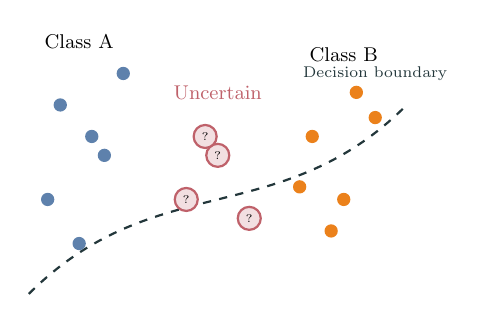
\begin{tikzpicture}[scale=0.8, transform shape]
% Decision boundary
\draw[thick, dashed, mDarkTeal] (0,-2) .. controls (2,0) and (4,-1) .. (6,1);

% Class A points (left of boundary)
\foreach \x/\y in {0.5/1, 1/0.5, 0.3/-0.5, 1.5/1.5, 0.8/-1.2, 1.2/0.2} {
  \fill[neutralcol] (\x,\y) circle (3pt);
}

% Class B points (right of boundary)
\foreach \x/\y in {4.5/0.5, 5/-0.5, 5.5/0.8, 4.8/-1, 5.2/1.2, 4.3/-0.3} {
  \fill[mLightBrown] (\x,\y) circle (3pt);
}

% Uncertain points (near boundary)
\foreach \x/\y in {2.5/-0.5, 3/0.2, 3.5/-0.8, 2.8/0.5} {
  \node[draw=alertcol, thick, circle, inner sep=2pt, fill=alertcol!20] at (\x,\y) {\tiny ?};
}

% Labels
\node[font=\small] at (0.8, 2) {Class A};
\node[font=\small] at (5, 1.8) {Class B};
\node[font=\small, alertcol] at (3, 1.2) {Uncertain};
\node[font=\scriptsize, mDarkTeal] at (5.5, 1.5) {Decision boundary};
\end{tikzpicture}
\end{center}

This requires a \textbf{trained model} -- surveys don't have one.\\
It is fundamentally model-driven, not design-driven.
\end{frame}

% ── Active learning is iterative ─────────────────────────────
\begin{frame}{Active learning is iterative; most surveys are not}

\begin{center}
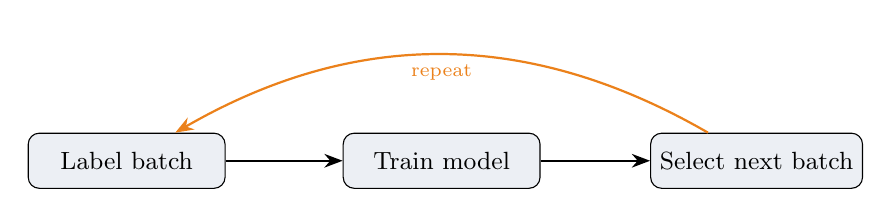
\begin{tikzpicture}[
  stagenode/.style={draw, rounded corners, fill=lightbg, minimum width=2.5cm, minimum height=0.7cm, align=center, font=\small},
  arrow/.style={-Stealth, thick}
]
\node[stagenode] (label) at (0,0) {Label batch};
\node[stagenode] (train) at (4,0) {Train model};
\node[stagenode] (select) at (8,0) {Select next batch};

\draw[arrow] (label) -- (train);
\draw[arrow] (train) -- (select);
\draw[arrow, mLightBrown] (select) to[bend right=30] node[below, font=\scriptsize] {repeat} (label);
\end{tikzpicture}
\end{center}

\vspace{1em}

Closest survey analogue: \textbf{adaptive/responsive survey designs}\\
(changing protocol based on accumulating data).

\vspace{1em}

Key difference: AL optimizes \textbf{model accuracy}.\\
Surveys optimize \textbf{population estimates}.
\end{frame}

% ── Sample size comparison ───────────────────────────────────
\begin{frame}{Sample size: formula vs.\ learning curve}

\begin{columns}[T]
\begin{column}{0.48\textwidth}
\textbf{Surveys}\\[0.5em]
$n$ determined \textbf{before} collection:\\[0.3em]
$\bullet$ Power analysis\\
$\bullet$ Margin of error\\
$\bullet$ Design effect\\[0.3em]
Clear stopping rule.
\end{column}

\begin{column}{0.48\textwidth}
\textbf{Active learning}\\[0.5em]
$n$ determined \textbf{during} collection:\\[0.3em]
$\bullet$ Monitor learning curve\\
$\bullet$ Stop when accuracy plateaus\\
$\bullet$ Or when budget runs out\\[0.3em]
No universal formula.
\end{column}
\end{columns}
\end{frame}

% ── What survey statisticians can bring ──────────────────────
\begin{frame}{What survey statisticians can bring to ML}

\begin{itemize}
  \item \textbf{Probability-based inference} -- AL has no guarantee\\
        that the labeled sample represents any population
  \item \textbf{Design-based estimation} -- Horvitz-Thompson,\\
        inclusion probabilities, design weights
  \item \textbf{Rigorous uncertainty quantification} -- confidence intervals\\
        tied to the sampling design
  \item \textbf{Decades of research} on nonresponse, coverage,\\
        and measurement error
\end{itemize}

\vspace{1em}

The ML field could benefit enormously from this expertise.
\end{frame}

% ── What ML can bring ────────────────────────────────────────
\begin{frame}{What ML can bring to survey statisticians}

\begin{itemize}
  \item \textbf{Adaptive, model-driven} sampling strategies
  \item Optimizing for \textbf{prediction} rather than just estimation
  \item \textbf{Active sampling for finite population inference}\\
        -- an emerging bridge between the fields
  \item Efficient use of limited labeling budgets
\end{itemize}

\vspace{1em}

The best path forward combines both traditions.
\end{frame}

% ── Discussion ───────────────────────────────────────────────
\begin{frame}[standout]
Discussion
\end{frame}

\begin{frame}{Discussion: Sampling}

\begin{enumerate}
  \item Where else do these fields talk past each other\\
        using the same vocabulary?

  \vspace{1em}

  \item In your work, when would you choose survey-style\\
        probability sampling over active learning -- or vice versa?
\end{enumerate}
\end{frame}

% ══════════════════════════════════════════════════════════════
% SECTION 7: Ethics
% ══════════════════════════════════════════════════════════════

\section{Ethics of Data Work}

\begin{frame}{The people who label your data}

Training data is produced by \textbf{people working for pay}.

\vspace{1em}

Ethical considerations:
\begin{itemize}
  \item \textbf{Wages:} Many crowdworkers earn below minimum wage
  \item \textbf{Benefits:} No health insurance, no job security
  \item \textbf{Harmful content:} Labelers exposed to violence, hate speech, abuse
  \item \textbf{Global dynamics:} Wealthy countries commission work;\\
        lower-income countries perform it
\end{itemize}
\end{frame}

% ── Exposure to harm ─────────────────────────────────────────
\begin{frame}{Labelers are exposed to harmful content}

Content moderation labelers routinely view:\\
violence, child abuse, self-harm, hate speech.

\vspace{1em}

\begin{itemize}
  \item Psychological harm is well-documented
  \item Workers often lack mental health support
  \item High turnover signals the toll this takes
\end{itemize}

\vspace{1em}

If your model requires labels on harmful content,\\
you have an obligation to protect labelers.
\end{frame}

% ── IRB and human subjects ───────────────────────────────────
\begin{frame}{Are labelers human subjects?}

Labeling tasks involve human judgment.\\
Should they require IRB/ethics board review?

\vspace{1em}

\begin{itemize}
  \item Labelers are performing a task, not being studied -- usually
  \item But research \textit{on} labelers (behavior, accuracy, bias)\\
        clearly involves human subjects
  \item The line is blurry; current regulations lag behind practice
\end{itemize}

\vspace{1em}

\textbf{Best practice:} Treat labelers with the same ethical\\
care you would give survey respondents.
\end{frame}

% ── Discussion ───────────────────────────────────────────────
\begin{frame}[standout]
Discussion
\end{frame}

\begin{frame}{Discussion: Ethics}

\begin{enumerate}
  \item What ethical obligations do ML teams have\\
        to the people who label their data?

  \vspace{1em}

  \item How should labeling tasks involving harmful content\\
        be designed to protect workers?
\end{enumerate}
\end{frame}

% ══════════════════════════════════════════════════════════════
% SECTION 8: Practical Advice
% ══════════════════════════════════════════════════════════════

\section{Practical Advice}

\begin{frame}{Concrete recommendations for better training data}

\begin{enumerate}
  \item \textbf{Treat labeling as measurement} -- apply instrument design principles
  \item \textbf{Pretest your task} -- pilot with a few annotators first
  \item \textbf{Document your design} -- task instructions, response options, labeler selection
  \item \textbf{Randomize} item order across annotators
  \item \textbf{Use multiple annotators} -- disagreement is signal, not noise
  \item \textbf{Collect paradata} -- time per item, revision patterns, confidence
  \item \textbf{Report who labeled} -- demographics, expertise, selection method
\end{enumerate}
\end{frame}

% ── Tools ────────────────────────────────────────────────────
\begin{frame}{Label collection tools}

\begin{description}
  \item[Open source:] Label Studio, Doccano, Prodigy
  \item[Commercial:] Scale AI, Labelbox, Amazon SageMaker Ground Truth
  \item[Crowd platforms:] Amazon MTurk, Prolific, Appen, Surge AI
\end{description}

\vspace{1em}

\textbf{Gaps:} Most tools do not collect paradata\\
(timing, revisions, annotator characteristics)\\
the way survey data collection platforms do.

\vspace{1em}

This is an opportunity for improvement.
\end{frame}

% ── What's missing ───────────────────────────────────────────
\begin{frame}{What the ML pipeline is missing from surveys}

\begin{itemize}
  \item \textbf{Standardized quality frameworks} (like TSE)
  \item \textbf{Pretesting protocols} for labeling instruments
  \item \textbf{Paradata collection} (timing, process data)
  \item \textbf{Transparent reporting} of data collection methods
  \item \textbf{Labeler selection documentation} (like survey sampling reports)
\end{itemize}

\vspace{1em}

\hfill \citep{eckman2024position}
\end{frame}

% ══════════════════════════════════════════════════════════════
% SECTION 9: Discussion / Closing
% ══════════════════════════════════════════════════════════════

\section{Discussion and Closing}

\begin{frame}[standout]
Open Discussion
\end{frame}

\begin{frame}{Questions for discussion}

\begin{enumerate}
  \item What aspects of survey methodology are most transferable\\
        to training data collection?

  \vspace{0.8em}

  \item What is different enough that new frameworks are needed?

  \vspace{0.8em}

  \item How should the survey research community engage\\
        with the growing demand for labeled data?
\end{enumerate}
\end{frame}

% ── Key takeaways ────────────────────────────────────────────
\begin{frame}{The one thing to remember}

\vspace{1em}

\textbf{Training data collection is data collection.}

\vspace{1em}

The same principles that make surveys reliable\\
--- careful design, transparent methods, rigorous\\
quality frameworks --- apply directly to labeling.

\vspace{1.5em}

Survey researchers are uniquely qualified\\
to improve this critical piece of the ML pipeline.
\end{frame}

% ── Thank you ────────────────────────────────────────────────
\begin{frame}{Thank you}
\textbf{Stephanie Eckman} -- seckman@umd.edu\\
\textbf{Frauke Kreuter} -- fkreuter@umd.edu

\vspace{2em}

Slides and references available at:\\
\url{https://github.com/seckman/training_data_course}

\vspace{1em}

\small Paper: \citet{eckman2024position}
\end{frame}

% ── References ───────────────────────────────────────────────
\begin{frame}[allowframebreaks]{References}
\small
\bibliography{references}
\end{frame}

\end{document}
